\section{Date: 2026-11-19}
\noindent \textbf{Series ID: JTS7100JOL} 

\noindent This series is titled Job Openings: Arts, Entertainment, and Recreation and has a frequency of Monthly. The units are Level in Thousands and the seasonal adjustment is Seasonally Adjusted.The observation start date is 2000-12-01 and the observation end date is 2026-09-01.The popularity of this series is 5. \\ 

\noindent \textbf{Series ID: MZMREAL} 

\noindent This series is titled Real MZM Money Stock (DISCONTINUED) and has a frequency of Monthly. The units are Billions of 1982-84 Dollars and the seasonal adjustment is Seasonally Adjusted.The observation start date is 1959-01-01 and the observation end date is 2021-01-01.The popularity of this series is 1. \\ 

\subsection{Raw Regression}
\noindent Regresses the two series against each other directly. A significant result here can come just as easily from both series sharing a long-run trend as from any real relationship.

\begin{center}
\begin{tabular}{lclc}
\toprule
\textbf{Dep. Variable:}          & value\_fred\_MZMREAL & \textbf{  R-squared:         } &     0.263   \\
\textbf{Model:}                  &         OLS          & \textbf{  Adj. R-squared:    } &     0.260   \\
\textbf{Method:}                 &    Least Squares     & \textbf{  F-statistic:       } &     85.83   \\
\textbf{Date:}                   &   Thu, 19 Nov 2026   & \textbf{  Prob (F-statistic):} &  1.16e-17   \\
\textbf{Time:}                   &       19:41:05       & \textbf{  Log-Likelihood:    } &   -2037.8   \\
\textbf{No. Observations:}       &           242        & \textbf{  AIC:               } &     4080.   \\
\textbf{Df Residuals:}           &           240        & \textbf{  BIC:               } &     4086.   \\
\textbf{Df Model:}               &             1        & \textbf{                     } &             \\
\textbf{Covariance Type:}        &      nonrobust       & \textbf{                     } &             \\
\bottomrule
\end{tabular}
\begin{tabular}{lcccccc}
                                 & \textbf{coef} & \textbf{std err} & \textbf{t} & \textbf{P$> |$t$|$} & \textbf{[0.025} & \textbf{0.975]}  \\
\midrule
\textbf{const}                   &    2858.4882  &      197.652     &    14.462  &         0.000        &     2469.135    &     3247.842     \\
\textbf{value\_fred\_JTS7100JOL} &      23.4806  &        2.535     &     9.264  &         0.000        &       18.488    &       28.473     \\
\bottomrule
\end{tabular}
\begin{tabular}{lclc}
\textbf{Omnibus:}       &  5.524 & \textbf{  Durbin-Watson:     } &    0.180  \\
\textbf{Prob(Omnibus):} &  0.063 & \textbf{  Jarque-Bera (JB):  } &    5.655  \\
\textbf{Skew:}          &  0.257 & \textbf{  Prob(JB):          } &   0.0592  \\
\textbf{Kurtosis:}      &  3.545 & \textbf{  Cond. No.          } &     217.  \\
\bottomrule
\end{tabular}
%\caption{OLS Regression Results}
\end{center}

Notes: \newline
 [1] Standard Errors assume that the covariance matrix of the errors is correctly specified.

\begin{figure}
\centering
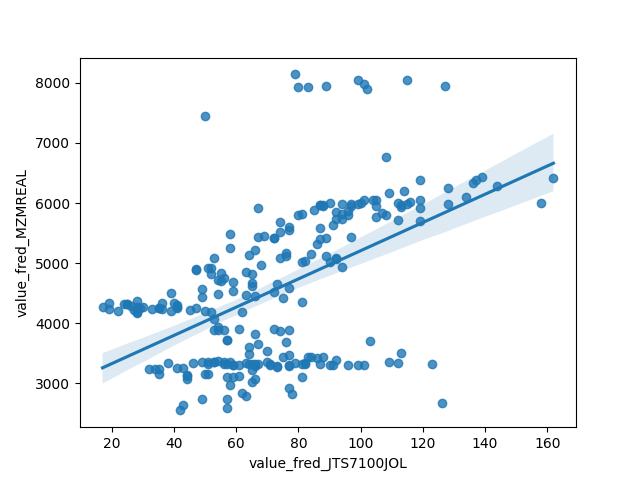
\includegraphics[scale = 0.9]{plots/plot_2026-11-19.png}
\caption{Raw Regression Plot for 2026-11-19}
\end{figure}
\newpage
\subsection{Detrended Regression}
\noindent Regresses the residuals of each series after removing its own linear time trend, so a shared trend can no longer drive the result on its own. A relationship that stays significant here is better evidence of a genuine link between the two series.

\begin{center}
\begin{tabular}{lclc}
\toprule
\textbf{Dep. Variable:}                     & value\_fred\_MZMREAL\_detrended & \textbf{  R-squared:         } &     0.001   \\
\textbf{Model:}                             &               OLS               & \textbf{  Adj. R-squared:    } &    -0.004   \\
\textbf{Method:}                            &          Least Squares          & \textbf{  F-statistic:       } &    0.1335   \\
\textbf{Date:}                              &         Thu, 19 Nov 2026        & \textbf{  Prob (F-statistic):} &    0.715    \\
\textbf{Time:}                              &             19:41:05            & \textbf{  Log-Likelihood:    } &   -1754.3   \\
\textbf{No. Observations:}                  &                 242             & \textbf{  AIC:               } &     3513.   \\
\textbf{Df Residuals:}                      &                 240             & \textbf{  BIC:               } &     3520.   \\
\textbf{Df Model:}                          &                   1             & \textbf{                     } &             \\
\textbf{Covariance Type:}                   &            nonrobust            & \textbf{                     } &             \\
\bottomrule
\end{tabular}
\begin{tabular}{lcccccc}
                                            & \textbf{coef} & \textbf{std err} & \textbf{t} & \textbf{P$> |$t$|$} & \textbf{[0.025} & \textbf{0.975]}  \\
\midrule
\textbf{const}                              &   -5.601e-11  &       21.979     & -2.55e-12  &         1.000        &      -43.296    &       43.296     \\
\textbf{value\_fred\_JTS7100JOL\_detrended} &       0.3378  &        0.924     &     0.365  &         0.715        &       -1.483    &        2.159     \\
\bottomrule
\end{tabular}
\begin{tabular}{lclc}
\textbf{Omnibus:}       & 141.914 & \textbf{  Durbin-Watson:     } &     0.032  \\
\textbf{Prob(Omnibus):} &   0.000 & \textbf{  Jarque-Bera (JB):  } &   734.824  \\
\textbf{Skew:}          &   2.445 & \textbf{  Prob(JB):          } & 2.72e-160  \\
\textbf{Kurtosis:}      &   9.997 & \textbf{  Cond. No.          } &      23.8  \\
\bottomrule
\end{tabular}
%\caption{OLS Regression Results}
\end{center}

Notes: \newline
 [1] Standard Errors assume that the covariance matrix of the errors is correctly specified.

\begin{figure}
\centering
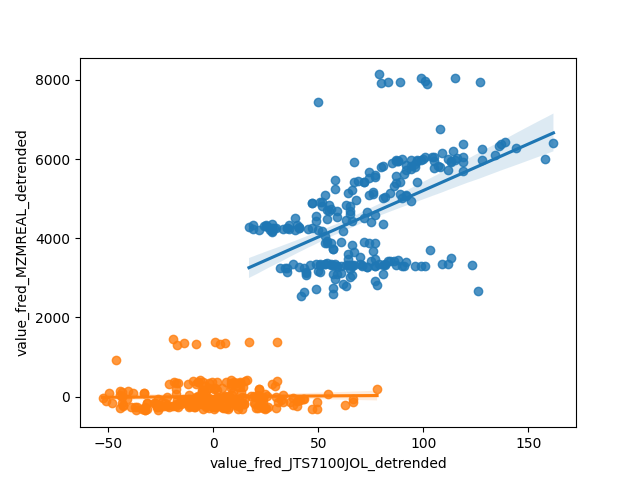
\includegraphics[scale = 0.9]{plots/plot_2026-11-19_detrended.png}
\caption{Detrended Regression Plot for 2026-11-19}
\end{figure}
\newpage
